\documentclass[11pt, letterpaper]{article}
\usepackage[utf8]{inputenc}
\usepackage[letterpaper, margin=1in]{geometry}
\usepackage{amsmath}
\usepackage{amssymb}
\usepackage{amsthm}
\usepackage{graphicx}
\usepackage[font=scriptsize]{caption}
\usepackage{subcaption}
\graphicspath{ {.} }
\captionsetup{justification=raggedright, singlelinecheck=false}


\title{Homework 2}
\author{Ryan Tang}
\date{September 29th 2022}

\begin{document}
\maketitle

\section{Exercise 10.1}
Since $G$ is the minimal I-map for $p(A, B, C, D, E, F, X)$, no other subgraph $G^{\prime}$ should contain any additional conditional-independence (CI) statements. Here, given the graph $G$, both $E$ and $F$ are independent of $A$ and $B$ given $X$. After marginalize out $X$, we need to add edges for $A \rightarrow E$, $B \rightarrow E$, $A \rightarrow F$, and $B \rightarrow F$. Otherwise, we will create an independence statement like $A \perp E$, which was not a part of the minimal I-map $G$.

\begin{figure*}[!h]
  \centering
  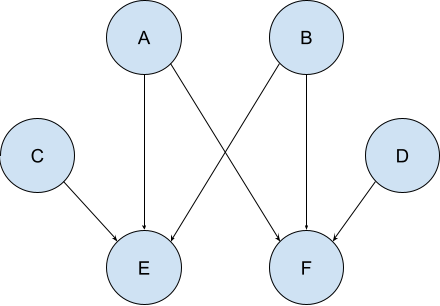
\includegraphics[width=0.4\textwidth]{hw2/10.1.png}
  \captionsetup{justification=centering}
  \caption{The new graph}
\end{figure*}

\section{Exercise 10.2}
\paragraph{(a)} Only $D$ is conditionally independent of $A$ given $B$; other nodes are not completely d-separated by B.
\paragraph{(b)} $\{C, E, F, H, I\}$ are conditionally independent of $A$ given $J$. Knowing $J$ opened the path between $A$ and $\{D, B\}$ instead.

\section{Exercise 10.3}
Given a graph $G$ with $V$ nodes, $t \in V$, $x_t$ is one of the node. And say $X_{-t}$ contains the set of nodes that consists of the Markov Blanket, $mb(x_t)$ of nodes $x_t$. Here we proof the full conditional of the Markov Blanket of node $x_t$ is given the following. Note, here we are only assuming the first-order Markov property within a DAG context.
\begin{proof}
\begin{align*}
    p(x_t|X_{-t}) &= \frac{p(x_t, X_{-t})}{p(X_{-t})} \\
        &\propto p(x_t, X_{ch(t)}, X_{pa(t)}, X_{copa(t)}) \\
        &= (\prod_{i \in pa(t)} p(x_i)) \cdot p(x_t|X_{pa(t)}) \cdot \prod_{j \in ch(t)} p(x_j|X_{pa(j)}) \\
        &\propto p(x_t|X_{pa(t)}) \cdot \prod_{j \in ch(t)} p(x_j|X_{pa(j)})
\end{align*}
\end{proof}

\section{Exercise 10.4}
\paragraph{(a)}
For nodes $X_{1:3}$, we only need one parameter for each to encode the binary outcome, 3 here. The hidden node needs one parameter per any possible combination of outcomes from $X_{1:3}$, $2^3=8$. For nodes, $X_{4:6}$, each of them needs one parameter for each possible outcome from the hidden node, $3*2=6$. Hence, we have $17$ parameters in the latent variable model.

\paragraph{(b)}
In contrast, the fully observed model with latent variable requires $59$ parameters because of the following: 1 parameter for each node in $X_{1:3}$. Node $X_4$ has 3 parents; thus, a table of $2^3=8$ parameters. Node $X_5$ has 4 parents, which requires a table of $2^4=16$ parameters. Lastly, node $X_6$ has 5 parents, which requires a table of $2^5=32$ parameters.

\paragraph{(c)}
The latent variable model is usually preferred because it has less number of parameters to estimate and can be estimated using the EM algorithm and MLE. It becomes more true when $n$ is small. However, it is all assumed that the latent variable model is a good representation of the underlying process to begin with.


\section{Exercise 10.5}
\paragraph{(a)}
\begin{align*}
    p(S=1|V=1) &= \frac{p(S=1, V=1)}{p(V=1)} \\
        &= \frac{p(V=1) \sum_i p(S=1|G=g_i)p(G=g_i)}{p(V=1)} \\
        &= \sum_i p(S=1|G=g_i)p(G=g_i) \\
        &= (1-\gamma)\alpha + (1-\beta)(1-\alpha)
\end{align*}

\paragraph{(b)}
$p(S=1|V=0)$ is equal to $p(S=1|V=1)$ because $V$ and $S$ are conditionally independent with each other as long as $R$ is not observed.

\paragraph{(c)}
The MLE result is $\delta=0, \alpha=\frac{1}{3}, \beta=0, \gamma=1$


\section{Exercise 10.6}
\paragraph{(a)}
Given the soft prior of season and a thin fish, we can express the our belief on $X_2$ as follow.
\begin{align*}
    p(X_2|X_1=x_1, X_4=thin) &\propto p(X_1=x_1)p(X_2|X_1=x_1)p(X4=thin|X2) \\
    p(X_2=Salmon|X_1=x_1, X_4=thin) &\propto 
        \begin{bmatrix}1/2 & 0 & 0 & 1/2\end{bmatrix}
        \begin{bmatrix}0.9 \\ 0.3 \\ 0.4 \\ 0.8\end{bmatrix}
        0.6 = 0.51 \\
    p(X_2=Sea Bass|X_1=x_1, X_4=thin) &\propto 
        \begin{bmatrix}1/2 & 0 & 0 & 1/2\end{bmatrix}
        \begin{bmatrix}0.1 \\ 0.7 \\ 0.6 \\ 0.2\end{bmatrix}
        0.05 = 0.0075 \\
    p(X_2|X_1=x_1, X_4=thin) &= \begin{bmatrix}0.9855 & 0.0145\end{bmatrix}
\end{align*}

\paragraph{(b)}
The query variable is the season node $X_1$ given the prior $p(X_1) = [1/4, 1/4, 1/4, 1/4]$, and we like to find
\begin{align*}
    p(X_1|X_3 = medium, X_4 = thin) &= \sum_{X_2} p(X_1, X_2 | X_3 = medium, X_4 = thin) \\
    p(X_1, X_2 | X_3 = medium, X_4 = thin) &\propto p(X_3 = medium, X_4 = thin | X_1, X_2)p(X_1, X_2)
\end{align*}
Therefore, I first iterated through all combinations of $X_1$ and $X_2$ to form the prior joint distribution. Then calculate the likelihood through the given data and the provided conditional probability tables (CPTs). Lastly, I integrated out the nuisance variable $X_2$ to get the conditional marginal of $X_1|X_3, X4$. The resulting belief is the following after normalization.
\[
    p(X_1|X_3 = medium, X_4 = thin) = [0.37, 0.13, 0.17, 0.33]
\]

\section{Exercise 10.7}
\paragraph{(a)}
Because the QMR network are bipartite graph, diseases are independent with each other. Hence, the following conditional. The unobserved symptoms don't enter into the picture at all.
\begin{align*}
    p(z_{1:3}|x_1, x_2, x_4) &\propto p(x_1, x_2, x_4|z_{1:3})p(z_{1:3})
        &= p(x_1|z_1) p(x_2|z_1, z_2) p(x_4|z_1, z_3) p(z_{1:3})
\end{align*}

\paragraph{(b)}
By the definition of a noisy-OR graph $G$ with hidden nodes $h_s$ and observed nodes $v_t$, the probability of seeing a disease with one symptom off is written as follows. $\theta_{st}$ is the probability of seeing a link $s \rightarrow t$ fails.
\begin{align*}
    p(h_s|v_t=0) &= \frac{p(v_t=0|h_s) p(h_s)}{p(v_t=0)} \\
        &= \frac{\theta_{st}^{\mathbb{I}(h_s=1)} p(h_s)}{1 + \theta_{st}^{\mathbb{I}(h_s=1)} p(h_s)} \\
\end{align*}
Therefore, when a symptom is off, the posterior is simply a damped version of its prior by the link-failure rate. In other words, we can directly ignore the off symptom and blend the failure rate into the prior.


\section{Exercise 10.8}
Essentially, when symptoms $\mathbf{f^{-}}$ are off, the posterior $p(\mathbf{d}|\mathbf{f^-})$ can be factorized because link-failure only happen when the hidden disease actually exists. There will be no link-failure $i \rightarrow j, \theta_{ij}$ when the hidden disease is off.
\begin{align*}
    p(\mathbf{d}|\mathbf{f^-}) &= p(d_1, d_2, \dots|\mathbf{f^-}) \\
        &= \prod_{i \in \mathbf{d}} p(d_i|\mathbf{f^-}) \\
        &= \prod_{i \in \mathbf{d}} \prod_{j \in f^-} \theta_{ij}^{\mathbb{I}(f^-=1)}
\end{align*}
Hence, we have the computation complexity $O(|\mathbf{d}||\mathbf{f^-}|)$.

\section{Exercise 11.8}
\paragraph{(a)}
Expectation is a linear operator; thus,
\begin{align*}
    \mathbb{E}[\mathbf{x}] &= \int \mathbf{x} \sum_k \pi_k \mathcal{N}(\mathbf{x}|\mathbf{\mu_k}, \mathbf{\Sigma_k}) d\mathbf{x} \\
        &= \sum_k \pi_k \int \mathbf{x} \mathcal{N}(\mathbf{x}|\mathbf{\mu_k}, \mathbf{\Sigma_k}) d\mathbf{x} \\
        &= \sum_k \pi_k \mathop{\mathbb{E}}_{\mathcal{N}_k}[\mathbf{x}] \\
        &= \sum_k \pi_k \mathbf{\mu_k}
\end{align*}

\paragraph{(b)}
Follow the same concept, we can derive the mixture covariance as follow.
\begin{align*}
    \text{cov}[\mathbf{x}] &= \mathbb{E}[\mathbf{x}\mathbf{x}^{\intercal}] - \mathbb{E}[\mathbf{x}]\mathbb{E}[\mathbf{x}]^{\intercal} \\
    \mathbb{E}[\mathbf{x}\mathbf{x}^{\intercal}]
        &= \int \mathbf{x}\mathbf{x}^{\intercal} \sum_k \pi_k \mathcal{N}(\mathbf{x}|\mathbf{\mu_k}, \mathbf{\Sigma_k}) d\mathbf{x} \\
        &= \sum_k \pi_k \int \mathbf{x}\mathbf{x}^{\intercal} \mathcal{N}(\mathbf{x}|\mathbf{\mu_k}, \mathbf{\Sigma_k}) d\mathbf{x} \\
        &= \sum_k \pi_k \mathop{\mathbb{E}}_{\mathcal{N}_k}[\mathbf{x}\mathbf{x}^{\intercal}] \\
\end{align*}
\begin{align*}
    \mathop{\mathbb{E}}_{\mathcal{N}_k}[\mathbf{x}\mathbf{x}^{\intercal}]
        &= \mathop{\text{var}}_{\mathcal{N}_k}[\mathbf{x}] + \mathop{\mathbb{E}}_{\mathcal{N}_k}[\mathbf{x}] \mathop{\mathbb{E}}_{\mathcal{N}_k}[\mathbf{x}]^{\intercal} \\
        &= \matbf{\Sigma_k} + \mathbf{\mu_k}\mathbf{\mu_k}^{\intercal}
\end{align*}
Therefore, the mixture covariance is given by
\begin{align*}
    \text{cov}[\mathbf{x}]
        &= \sum_k \pi_k (\matbf{\Sigma_k} + \mathbf{\mu_k}\mathbf{\mu_k}^{\intercal})
           - \mathbb{E}[\mathbf{x}]\mathbb{E}[\mathbf{x}]^{\intercal}
\end{align*}

\section{Exercise 11.11}
Given a 1d Gaussian mixture model (GMM) with $k$ labels, $\mathbf{z} \in {\mathbb{R}^k}$ and 1d feature $x \in \mathbb{R}$, the join density $p(x, \mathbf{z}|\boldsymbol{\theta})$ has an exponential family form. For each class-label, the Gaussian distribution is parameterized by $\theta_i = [\mu_i, \sigma_i^2], \forall i \in k$.
\begin{proof}
\begin{align*}
    p(\mathbf{z}) &= \prod_{i \in k} \pi_i^{z_i} \\
    p(x | \mathbf{z}, \boldsymbol{\theta}) &= \prod_{i \in k} [\mathcal{N}(x|\mu_i, \sigma_i^2)]^{z_i} \\
    p(x, \mathbf{z}|\boldsymbol{\theta}) &= p(x | \mathbf{z}, \boldsymbol{\theta}) p(\mathbf{z}) \\
        &= \prod_{i \in k} [\pi_i \mathcal{N}(x|\mu_i, \sigma_i^2)]^{z_i} \\
        &= \prod_{i \in k} [\frac{\pi_i}{\sigma_i \sqrt{2\pi}} \exp[-\frac{1}{2} (\frac{x-\mu_i}{\sigma_i})^2]]^{z_i} \\
        &= \prod_{i \in k} \exp[\frac{-1}{2\sigma_i^2}x^2 + \frac{1}{\sigma_i^2}x - A_{i}(\boldsymbol{\eta_i}, \pi_i)]^{z_i} \\
        &= \prod_{i \in k} \exp[\boldsymbol{\eta_i}^{\intercal}\boldsymbol{t}(x) - A_{i}(\boldsymbol{\eta_i}, \pi_i)]^{z_i}
            && \boldsymbol{\eta} = \begin{bmatrix}\frac{\mu_i}{\sigma_i^2} & -\frac{1}{2\sigma_i^2}\end{bmatrix}^{\intercal} \\
        &= \exp[\sum_{i \in k} z_i (\boldsymbol{\eta_i}^{\intercal}\boldsymbol{t}(x) - A_{i}(\boldsymbol{\eta_i}, \pi_i))]
            && \boldsymbol{t}(x) = \begin{bmatrix}x & x^2\end{bmatrix}^{\intercal} \\
\end{align*}
\end{proof}
Hence, we can see it is a weighted sum of the exponential form.

\end{document}